% Options for packages loaded elsewhere
\PassOptionsToPackage{unicode}{hyperref}
\PassOptionsToPackage{hyphens}{url}
\PassOptionsToPackage{dvipsnames,svgnames,x11names}{xcolor}
%
\documentclass[
  letterpaper,
  DIV=11,
  numbers=noendperiod]{scrartcl}

\usepackage{amsmath,amssymb}
\usepackage{iftex}
\ifPDFTeX
  \usepackage[T1]{fontenc}
  \usepackage[utf8]{inputenc}
  \usepackage{textcomp} % provide euro and other symbols
\else % if luatex or xetex
  \usepackage{unicode-math}
  \defaultfontfeatures{Scale=MatchLowercase}
  \defaultfontfeatures[\rmfamily]{Ligatures=TeX,Scale=1}
\fi
\usepackage{lmodern}
\ifPDFTeX\else  
    % xetex/luatex font selection
\fi
% Use upquote if available, for straight quotes in verbatim environments
\IfFileExists{upquote.sty}{\usepackage{upquote}}{}
\IfFileExists{microtype.sty}{% use microtype if available
  \usepackage[]{microtype}
  \UseMicrotypeSet[protrusion]{basicmath} % disable protrusion for tt fonts
}{}
\makeatletter
\@ifundefined{KOMAClassName}{% if non-KOMA class
  \IfFileExists{parskip.sty}{%
    \usepackage{parskip}
  }{% else
    \setlength{\parindent}{0pt}
    \setlength{\parskip}{6pt plus 2pt minus 1pt}}
}{% if KOMA class
  \KOMAoptions{parskip=half}}
\makeatother
\usepackage{xcolor}
\setlength{\emergencystretch}{3em} % prevent overfull lines
\setcounter{secnumdepth}{-\maxdimen} % remove section numbering
% Make \paragraph and \subparagraph free-standing
\ifx\paragraph\undefined\else
  \let\oldparagraph\paragraph
  \renewcommand{\paragraph}[1]{\oldparagraph{#1}\mbox{}}
\fi
\ifx\subparagraph\undefined\else
  \let\oldsubparagraph\subparagraph
  \renewcommand{\subparagraph}[1]{\oldsubparagraph{#1}\mbox{}}
\fi

\usepackage{color}
\usepackage{fancyvrb}
\newcommand{\VerbBar}{|}
\newcommand{\VERB}{\Verb[commandchars=\\\{\}]}
\DefineVerbatimEnvironment{Highlighting}{Verbatim}{commandchars=\\\{\}}
% Add ',fontsize=\small' for more characters per line
\usepackage{framed}
\definecolor{shadecolor}{RGB}{241,243,245}
\newenvironment{Shaded}{\begin{snugshade}}{\end{snugshade}}
\newcommand{\AlertTok}[1]{\textcolor[rgb]{0.68,0.00,0.00}{#1}}
\newcommand{\AnnotationTok}[1]{\textcolor[rgb]{0.37,0.37,0.37}{#1}}
\newcommand{\AttributeTok}[1]{\textcolor[rgb]{0.40,0.45,0.13}{#1}}
\newcommand{\BaseNTok}[1]{\textcolor[rgb]{0.68,0.00,0.00}{#1}}
\newcommand{\BuiltInTok}[1]{\textcolor[rgb]{0.00,0.23,0.31}{#1}}
\newcommand{\CharTok}[1]{\textcolor[rgb]{0.13,0.47,0.30}{#1}}
\newcommand{\CommentTok}[1]{\textcolor[rgb]{0.37,0.37,0.37}{#1}}
\newcommand{\CommentVarTok}[1]{\textcolor[rgb]{0.37,0.37,0.37}{\textit{#1}}}
\newcommand{\ConstantTok}[1]{\textcolor[rgb]{0.56,0.35,0.01}{#1}}
\newcommand{\ControlFlowTok}[1]{\textcolor[rgb]{0.00,0.23,0.31}{#1}}
\newcommand{\DataTypeTok}[1]{\textcolor[rgb]{0.68,0.00,0.00}{#1}}
\newcommand{\DecValTok}[1]{\textcolor[rgb]{0.68,0.00,0.00}{#1}}
\newcommand{\DocumentationTok}[1]{\textcolor[rgb]{0.37,0.37,0.37}{\textit{#1}}}
\newcommand{\ErrorTok}[1]{\textcolor[rgb]{0.68,0.00,0.00}{#1}}
\newcommand{\ExtensionTok}[1]{\textcolor[rgb]{0.00,0.23,0.31}{#1}}
\newcommand{\FloatTok}[1]{\textcolor[rgb]{0.68,0.00,0.00}{#1}}
\newcommand{\FunctionTok}[1]{\textcolor[rgb]{0.28,0.35,0.67}{#1}}
\newcommand{\ImportTok}[1]{\textcolor[rgb]{0.00,0.46,0.62}{#1}}
\newcommand{\InformationTok}[1]{\textcolor[rgb]{0.37,0.37,0.37}{#1}}
\newcommand{\KeywordTok}[1]{\textcolor[rgb]{0.00,0.23,0.31}{#1}}
\newcommand{\NormalTok}[1]{\textcolor[rgb]{0.00,0.23,0.31}{#1}}
\newcommand{\OperatorTok}[1]{\textcolor[rgb]{0.37,0.37,0.37}{#1}}
\newcommand{\OtherTok}[1]{\textcolor[rgb]{0.00,0.23,0.31}{#1}}
\newcommand{\PreprocessorTok}[1]{\textcolor[rgb]{0.68,0.00,0.00}{#1}}
\newcommand{\RegionMarkerTok}[1]{\textcolor[rgb]{0.00,0.23,0.31}{#1}}
\newcommand{\SpecialCharTok}[1]{\textcolor[rgb]{0.37,0.37,0.37}{#1}}
\newcommand{\SpecialStringTok}[1]{\textcolor[rgb]{0.13,0.47,0.30}{#1}}
\newcommand{\StringTok}[1]{\textcolor[rgb]{0.13,0.47,0.30}{#1}}
\newcommand{\VariableTok}[1]{\textcolor[rgb]{0.07,0.07,0.07}{#1}}
\newcommand{\VerbatimStringTok}[1]{\textcolor[rgb]{0.13,0.47,0.30}{#1}}
\newcommand{\WarningTok}[1]{\textcolor[rgb]{0.37,0.37,0.37}{\textit{#1}}}

\providecommand{\tightlist}{%
  \setlength{\itemsep}{0pt}\setlength{\parskip}{0pt}}\usepackage{longtable,booktabs,array}
\usepackage{calc} % for calculating minipage widths
% Correct order of tables after \paragraph or \subparagraph
\usepackage{etoolbox}
\makeatletter
\patchcmd\longtable{\par}{\if@noskipsec\mbox{}\fi\par}{}{}
\makeatother
% Allow footnotes in longtable head/foot
\IfFileExists{footnotehyper.sty}{\usepackage{footnotehyper}}{\usepackage{footnote}}
\makesavenoteenv{longtable}
\usepackage{graphicx}
\makeatletter
\def\maxwidth{\ifdim\Gin@nat@width>\linewidth\linewidth\else\Gin@nat@width\fi}
\def\maxheight{\ifdim\Gin@nat@height>\textheight\textheight\else\Gin@nat@height\fi}
\makeatother
% Scale images if necessary, so that they will not overflow the page
% margins by default, and it is still possible to overwrite the defaults
% using explicit options in \includegraphics[width, height, ...]{}
\setkeys{Gin}{width=\maxwidth,height=\maxheight,keepaspectratio}
% Set default figure placement to htbp
\makeatletter
\def\fps@figure{htbp}
\makeatother

\KOMAoption{captions}{tableheading}
\makeatletter
\makeatother
\makeatletter
\makeatother
\makeatletter
\@ifpackageloaded{caption}{}{\usepackage{caption}}
\AtBeginDocument{%
\ifdefined\contentsname
  \renewcommand*\contentsname{Table of contents}
\else
  \newcommand\contentsname{Table of contents}
\fi
\ifdefined\listfigurename
  \renewcommand*\listfigurename{List of Figures}
\else
  \newcommand\listfigurename{List of Figures}
\fi
\ifdefined\listtablename
  \renewcommand*\listtablename{List of Tables}
\else
  \newcommand\listtablename{List of Tables}
\fi
\ifdefined\figurename
  \renewcommand*\figurename{Figure}
\else
  \newcommand\figurename{Figure}
\fi
\ifdefined\tablename
  \renewcommand*\tablename{Table}
\else
  \newcommand\tablename{Table}
\fi
}
\@ifpackageloaded{float}{}{\usepackage{float}}
\floatstyle{ruled}
\@ifundefined{c@chapter}{\newfloat{codelisting}{h}{lop}}{\newfloat{codelisting}{h}{lop}[chapter]}
\floatname{codelisting}{Listing}
\newcommand*\listoflistings{\listof{codelisting}{List of Listings}}
\makeatother
\makeatletter
\@ifpackageloaded{caption}{}{\usepackage{caption}}
\@ifpackageloaded{subcaption}{}{\usepackage{subcaption}}
\makeatother
\makeatletter
\@ifpackageloaded{tcolorbox}{}{\usepackage[skins,breakable]{tcolorbox}}
\makeatother
\makeatletter
\@ifundefined{shadecolor}{\definecolor{shadecolor}{rgb}{.97, .97, .97}}
\makeatother
\makeatletter
\makeatother
\makeatletter
\makeatother
\ifLuaTeX
  \usepackage{selnolig}  % disable illegal ligatures
\fi
\IfFileExists{bookmark.sty}{\usepackage{bookmark}}{\usepackage{hyperref}}
\IfFileExists{xurl.sty}{\usepackage{xurl}}{} % add URL line breaks if available
\urlstyle{same} % disable monospaced font for URLs
\hypersetup{
  pdftitle={Metabolomics\_analysis\_tools Tutorials},
  colorlinks=true,
  linkcolor={blue},
  filecolor={Maroon},
  citecolor={Blue},
  urlcolor={Blue},
  pdfcreator={LaTeX via pandoc}}

\title{Metabolomics\_analysis\_tools Tutorials}
\author{}
\date{}

\begin{document}
\maketitle
\ifdefined\Shaded\renewenvironment{Shaded}{\begin{tcolorbox}[boxrule=0pt, frame hidden, borderline west={3pt}{0pt}{shadecolor}, sharp corners, interior hidden, enhanced, breakable]}{\end{tcolorbox}}\fi

\textbf{Introduction to the Metabolomics analysis tools}

The goal of this project is to implement a Python based pipeline or
package related to metabolomics data analysis. I am currently working
with targeted metabolomics data in my lab, and it will be helpful with
my work to develop a package that contains some very common metabolomics
data analysis tools, including:

data transformation data normalization data scaling common statistical
analyses including PCA, MA plot and Volcano plot. Even though there are
lots of packages available for the functions mentioned above,
implementing them myself will help me understand those functions better
and help me do a better analysis job hopefully.

\textbf{Goal of the tutorial}

The goal of this tutorial is to show step by step how to install and use
this package to perform data processing and statistical analyses
functions in this tool, and also a bit on how to read the results
generated from the analyses functions.

\textbf{Example data description}

Targeted metabolomics data Retrieve metabolites concentration data from
(https://www.metaboanalyst.ca/MetaboAnalyst/upload/StatUploadView.xhtml
or from https://www.ebi.ac.uk/metabolights/search?) (Metabolights)

A data file with metabolites concentration profile will contain a matrix
with metabolites names and metabolites concentrations on each row for
each sample. This file will be provided by the user, I will have data
for testing

\textbf{Step by step installation and running}

Let's get started! First, we need to install the package.\\
Steps: 1. Git clone or download the github folder;\\
2. Open the terminal, and go to this folder;\\
3. Enter\\
\texttt{pip\ install\ dist/metabolomics\_analysis\_tools-0.1.0.tar.gz}
to install the package locally;

Then, we can import functions we will use for this demo from the package
metabolomics\_analysis\_tools@import\_functions.

\hypertarget{import_functions}{}
\begin{Shaded}
\begin{Highlighting}[]
\ImportTok{import}\NormalTok{ metabolomics\_analysis\_tools.data\_preprocessing.data\_reading }\ImportTok{as}\NormalTok{ dr}
\ImportTok{import}\NormalTok{ metabolomics\_analysis\_tools.data\_preprocessing.normalization }\ImportTok{as}\NormalTok{ dn}
\ImportTok{import}\NormalTok{ metabolomics\_analysis\_tools.stats\_analyses.analyses }\ImportTok{as}\NormalTok{ sa}
\ImportTok{import}\NormalTok{ warnings}
\NormalTok{warnings.filterwarnings(}\StringTok{\textquotesingle{}ignore\textquotesingle{}}\NormalTok{)}
\end{Highlighting}
\end{Shaded}

\begin{enumerate}
\def\labelenumi{\arabic{enumi}.}
\tightlist
\item
  Then we can use the data\_reading module to read in the data, by
  default it will read in the data from the resources/test\_dataset
  folder in the package.\\
  We can also use the data\_reading module to read in the data from a
  custom path, by passing the path as an argument to the
  read\_data\_file function (file\_path=`path/to/file.csv').\\
  The read\_data\_file function will return a pandas dataframe.
\end{enumerate}

\begin{Shaded}
\begin{Highlighting}[]
\NormalTok{df}\OperatorTok{=}\NormalTok{dr.read\_data\_file()}
\NormalTok{df.head()}
\end{Highlighting}
\end{Shaded}

\begin{verbatim}
data read successfully
the shape of the dataframe is:  (77, 65)
\end{verbatim}

\hypertarget{read_data}{}
\begin{tabular}{llllllllllllllllllllllllllllllllllllllllllllllllllllllllllllllllll}
\toprule
{} &   Patient ID & Muscle loss & 1,6-Anhydro-beta-D-glucose & 1-Methylnicotinamide & 2-Aminobutyrate & 2-Hydroxyisobutyrate & 2-Oxoglutarate & 3-Aminoisobutyrate & 3-Hydroxybutyrate & 3-Hydroxyisovalerate & 3-Indoxylsulfate & 4-Hydroxyphenylacetate & Acetate & Acetone & Adipate &  Alanine & Asparagine & Betaine & Carnitine &   Citrate & Creatine & Creatinine & Dimethylamine & Ethanolamine & Formate &  Fucose & Fumarate &  Glucose & Glutamine &  Glycine & Glycolate & Guanidoacetate & Hippurate & Histidine & Hypoxanthine & Isoleucine &  Lactate & Leucine &  Lysine & Methylamine & Methylguanidine & N,N-Dimethylglycine & O-Acetylcarnitine & Pantothenate & Pyroglutamate & Pyruvate & Quinolinate &   Serine & Succinate & Sucrose & Tartrate &  Taurine & Threonine & Trigonelline & Trimethylamine N-oxide & Tryptophan & Tyrosine &  Uracil &  Valine &   Xylose & cis-Aconitate & myo-Inositol & trans-Aconitate & pi-Methylhistidine & tau-Methylhistidine \\
\midrule
0 &      PIF\_178 &    cachexic &                      40.85 &                65.37 &           18.73 &                26.05 &          71.52 &             1480.3 &             56.83 &                10.07 &            566.8 &                  120.3 &  126.47 &    9.49 &   38.09 &   314.19 &     159.17 &  109.95 &    265.07 &    3714.5 &   196.37 &    16481.6 &         632.7 &       645.48 &  441.42 &  336.97 &     7.69 &   395.44 &    871.31 &  2038.56 &     685.4 &         154.47 &    4582.5 &    925.19 &        97.51 &       5.58 &    106.7 &    42.1 &  146.94 &       52.46 &            9.97 &               23.34 &             52.98 &        25.79 &        437.03 &    21.12 &      165.67 &   284.29 &    154.47 &   45.15 &    97.51 &  1919.85 &    184.93 &       943.88 &                2121.76 &     259.82 &   290.03 &  111.05 &   86.49 &    72.24 &        237.46 &       135.64 &           51.94 &             157.59 &              160.77 \\
1 &      PIF\_087 &    cachexic &                      62.18 &               340.36 &           24.29 &                41.68 &          67.36 &             116.75 &             43.82 &                79.84 &           368.71 &                 432.68 &  212.72 &   11.82 &  327.01 &   871.31 &     157.59 &  244.69 &     120.3 &   2617.57 &   212.72 &   15835.35 &        607.89 &       487.85 &  252.14 &  198.34 &    18.92 &  8690.62 &    601.85 &  1107.65 &    651.97 &         109.95 &   1737.15 &    845.56 &        82.27 &       8.17 &   368.71 &   77.48 &  284.29 &       23.57 &            7.69 &               87.36 &              50.4 &       186.79 &        437.03 &    36.97 &       72.97 &   391.51 &    244.69 &  459.44 &    32.79 &  1261.43 &    198.34 &       208.51 &                 639.06 &       83.1 &   167.34 &   46.99 &  109.95 &   192.48 &        333.62 &       376.15 &          217.02 &             307.97 &              130.32 \\
2 &      PIF\_090 &    cachexic &                     270.43 &                64.72 &           12.18 &                65.37 &          23.81 &               14.3 &              5.64 &                23.34 &           665.14 &                 292.95 &  314.19 &    4.44 &  131.63 &   464.05 &      89.12 &  116.75 &     25.03 &    862.64 &   221.41 &   24587.66 &         735.1 &       407.48 &  249.64 &  186.79 &      7.1 &  1352.89 &    301.87 &   620.17 &    141.17 &         183.09 &   4315.64 &    284.29 &       114.43 &        9.3 &   749.95 &    31.5 &   97.51 &       18.73 &            4.66 &               24.53 &              5.58 &       145.47 &        713.37 &    29.37 &      192.48 &   295.89 &    142.59 &  160.77 &    16.28 &  4272.69 &    109.95 &       192.48 &                1152.86 &      82.27 &    60.34 &    31.5 &   59.15 &  2164.62 &         330.3 &        86.49 &           58.56 &             145.47 &               83.93 \\
3 &  NETL\_005\_V1 &    cachexic &                     154.47 &                52.98 &          172.43 &                74.44 &        1199.91 &             555.57 &            175.91 &                25.03 &           411.58 &                 214.86 &   37.34 &  206.44 &  144.03 &   589.93 &     273.14 &  278.66 &    200.34 &  13629.61 &    85.63 &   20952.22 &       1064.22 &       820.57 &  468.72 &  407.48 &    96.54 &   862.64 &   1685.81 &  5064.45 &     70.81 &         102.51 &    757.48 &   1043.15 &       223.63 &      37.71 &   368.71 &  103.54 &  290.03 &       48.91 &          141.17 &               40.04 &            254.68 &        42.52 &         566.8 &    64.07 &       86.49 &  1248.88 &    144.03 &  111.05 &   837.15 &  1525.38 &    376.15 &       992.27 &                1450.99 &      235.1 &   323.76 &   30.57 &  102.51 &   125.21 &       1863.11 &       247.15 &           75.94 &             249.64 &              254.68 \\
4 &      PIF\_115 &    cachexic &                       22.2 &                 73.7 &           15.64 &                83.93 &          33.12 &              29.67 &             76.71 &                69.41 &           165.67 &                  97.51 &  407.48 &   44.26 &   15.03 &  1118.79 &      42.52 &  391.51 &     84.77 &    854.06 &   105.64 &    6768.26 &        242.26 &       365.04 &  114.43 &   26.05 &    19.69 &  6836.29 &    432.68 &   395.44 &     26.58 &          52.98 &   1152.86 &    327.01 &        66.69 &      40.04 &  3640.95 &  101.49 &  122.73 &       27.94 &            5.31 &               46.06 &              45.6 &        74.44 &        184.93 &     12.3 &       38.09 &   206.44 &     68.72 &   75.19 &     4.53 &   468.72 &     64.07 &        86.49 &                 172.43 &     103.54 &   142.59 &   44.26 &  160.77 &   186.79 &        101.49 &       749.95 &           98.49 &              84.77 &               79.84 \\
\bottomrule
\end{tabular}

\begin{enumerate}
\def\labelenumi{\arabic{enumi}.}
\setcounter{enumi}{1}
\tightlist
\item
  Next we can use the normalization module to normalize the data, here
  we will use the median normalization method
  normalized\_data=dn.normalize\_by\_median(df).\\
  We can have a look at the first 5 rows of the normalized data
  normalized\_data.head().\\
\end{enumerate}

\begin{Shaded}
\begin{Highlighting}[]
\NormalTok{normalized\_data}\OperatorTok{=}\NormalTok{dn.normalize\_by\_median(df)}
\NormalTok{normalized\_data.head()}
\end{Highlighting}
\end{Shaded}

\hypertarget{normalize_data}{}
\begin{tabular}{llllllllllllllllllllllllllllllllllllllllllllllllllllllllllllllllll}
\toprule
{} &   Patient ID & Muscle loss & 1,6-Anhydro-beta-D-glucose & 1-Methylnicotinamide & 2-Aminobutyrate & 2-Hydroxyisobutyrate & 2-Oxoglutarate & 3-Aminoisobutyrate & 3-Hydroxybutyrate & 3-Hydroxyisovalerate & 3-Indoxylsulfate & 4-Hydroxyphenylacetate &    Acetate &    Acetone &    Adipate &   Alanine & Asparagine &   Betaine &  Carnitine &   Citrate &  Creatine & Creatinine & Dimethylamine & Ethanolamine &   Formate &    Fucose &   Fumarate &    Glucose & Glutamine &   Glycine & Glycolate & Guanidoacetate & Hippurate & Histidine & Hypoxanthine & Isoleucine &    Lactate &   Leucine &    Lysine & Methylamine & Methylguanidine & N,N-Dimethylglycine & O-Acetylcarnitine & Pantothenate & Pyroglutamate &  Pyruvate & Quinolinate &    Serine & Succinate &    Sucrose &   Tartrate &    Taurine & Threonine & Trigonelline & Trimethylamine N-oxide & Tryptophan &  Tyrosine &    Uracil &    Valine &    Xylose & cis-Aconitate & myo-Inositol & trans-Aconitate & pi-Methylhistidine & tau-Methylhistidine \\
\midrule
0 &      PIF\_178 &    cachexic &                   0.895833 &             1.786066 &         1.78551 &             0.802526 &       1.296827 &          65.355408 &          4.857265 &              0.80239 &         3.935291 &               1.715875 &    3.18966 &    1.33662 &    3.74165 &  1.616037 &    3.78076 &  1.698857 &  11.132717 &  2.075082 &  4.436737 &   2.159765 &      2.075107 &     3.158235 &   4.61833 &  5.473847 &    1.87561 &   1.877594 &  3.857402 &  3.857402 &  5.259362 &       2.386743 &  3.743414 &  5.312299 &     2.435315 &   0.778243 &   1.310006 &  2.203035 &  2.116986 &    3.561439 &        1.270064 &            1.061874 &          4.619006 &     1.138631 &      2.773209 &  1.569094 &    3.221898 &  1.993758 &  5.002267 &   1.105263 &   7.535549 &   7.690474 &  2.886374 &     8.248536 &               5.529016 &   5.529262 &  4.806596 &  4.054399 &  2.611413 &  1.433333 &       1.84049 &     1.733197 &        1.935171 &           0.970442 &            2.339494 \\
1 &      PIF\_087 &    cachexic &                   1.363596 &             9.299454 &        2.315539 &             1.284042 &       1.221396 &           5.154525 &          3.745299 &             6.361753 &         2.559953 &               6.171445 &   5.364943 &   1.664789 &   32.12279 &  4.481586 &    3.74323 &  3.780748 &   5.052499 &  1.462289 &  4.806146 &    2.07508 &      1.993736 &     2.386975 &     2.638 &  3.221897 &   4.614634 &  41.264043 &  2.664468 &  2.095917 &  5.002839 &       1.698857 &  1.419066 &  4.855076 &     2.054695 &    1.13947 &   4.526826 &  4.054422 &  4.095808 &    1.600136 &        0.979618 &            3.974522 &          4.394071 &     8.246799 &      2.773209 &  2.746657 &    1.419098 &  2.745704 &  7.923899 &  11.247001 &   2.534003 &   5.052996 &  3.095677 &     1.822162 &               1.665303 &   1.768461 &  2.773285 &   1.71559 &  3.319746 &  3.819048 &      2.585801 &     4.806415 &        8.085693 &           1.896484 &            1.896391 \\
2 &      PIF\_090 &    cachexic &                   5.930482 &             1.768306 &        1.161106 &             2.013863 &       0.431732 &           0.631347 &          0.482051 &             1.859761 &         4.618066 &               4.178434 &   7.924086 &   0.625352 &  12.930255 &  2.386843 &   2.116865 &  1.803925 &   1.051239 &  0.481908 &  5.002485 &   3.221991 &      2.410954 &     1.993737 &  2.611843 &  3.034276 &   1.731707 &   6.423674 &  1.336418 &  1.173498 &  1.083257 &       2.828956 &  3.525418 &   1.63235 &     2.857892 &   1.297071 &   9.207489 &  1.648352 &  1.404841 &    1.271555 &        0.593631 &            1.116015 &          0.486486 &     6.422517 &      4.526747 &  2.182021 &    3.743291 &   2.07511 &  4.617552 &   3.935618 &   1.258114 &  17.115406 &  1.716092 &     1.682076 &               3.004195 &   1.750798 &       1.0 &  1.150055 &   1.78593 &  42.94881 &      2.560068 &     1.105162 &        2.181818 &           0.895806 &            1.221333 \\
3 &  NETL\_005\_V1 &    cachexic &                     3.3875 &             1.447541 &        16.43756 &             2.293284 &      21.757208 &          24.528477 &         15.035043 &             1.994422 &         2.857599 &               3.064613 &    0.94174 &  29.076056 &   14.14833 &  3.034307 &   6.487886 &  4.305624 &   8.414112 &  7.614095 &  1.934704 &     2.7456 &       3.49039 &     4.014923 &  4.903955 &  6.619233 &  23.546341 &   4.095912 &  7.463299 &   9.58305 &  0.543355 &         1.5839 &   0.61878 &  5.989607 &     5.585165 &   5.259414 &   4.526826 &  5.418106 &  4.178505 &    3.320434 &       17.983439 &            1.821656 &          22.20401 &     1.877263 &      3.596675 &   4.76003 &     1.68203 &  8.758538 &  4.664184 &   2.718482 &  64.694745 &   6.110319 &  5.870922 &     8.671415 &               3.781081 &   5.003192 &  5.365595 &  1.116101 &  3.095109 &  2.484325 &     14.440474 &     3.158063 &        2.829359 &           1.537287 &            3.706054 \\
4 &      PIF\_115 &    cachexic &                   0.486842 &             2.013661 &        1.490944 &             2.585644 &       0.600544 &           1.309934 &           6.55641 &             5.530677 &         1.150246 &               1.390814 &  10.276923 &   6.233803 &   1.476424 &  5.754501 &   1.009976 &  6.049289 &   3.560269 &  0.477115 &  2.386805 &   0.886919 &      0.794556 &     1.786085 &  1.197217 &  0.423164 &   4.802439 &  32.459475 &   1.91553 &  0.748259 &  0.203959 &       0.818603 &  0.941764 &  1.877641 &     1.665584 &   5.584379 &  44.701657 &  5.310832 &  1.768189 &    1.896809 &        0.676433 &            2.095541 &          3.975588 &     3.286534 &      1.173488 &  0.913819 &    0.740762 &  1.447787 &  2.225389 &   1.840636 &   0.350077 &   1.877584 &       1.0 &     0.755833 &               0.449329 &   2.203448 &  2.363109 &  1.615918 &  4.854167 &  3.706151 &      0.786622 &     9.582801 &        3.669523 &           0.522015 &            1.161816 \\
\bottomrule
\end{tabular}

\begin{enumerate}
\def\labelenumi{\arabic{enumi}.}
\setcounter{enumi}{2}
\tightlist
\item
  (a)We can use the analyses module to perform statistical analyses on
  the data.\\
  Here we will first perform a PCA analysis on the data to see if there
  are any patterns in the data.\\
  The PCA\_analysis function will return a pandas dataframe containing
  the principal components
  principal\_components=sa.PCA\_analysis(normalized\_data).
\end{enumerate}

\begin{Shaded}
\begin{Highlighting}[]
\NormalTok{principal\_components}\OperatorTok{=}\NormalTok{sa.PCA\_analysis(normalized\_data)}
\end{Highlighting}
\end{Shaded}

\begin{figure}[H]

{\centering 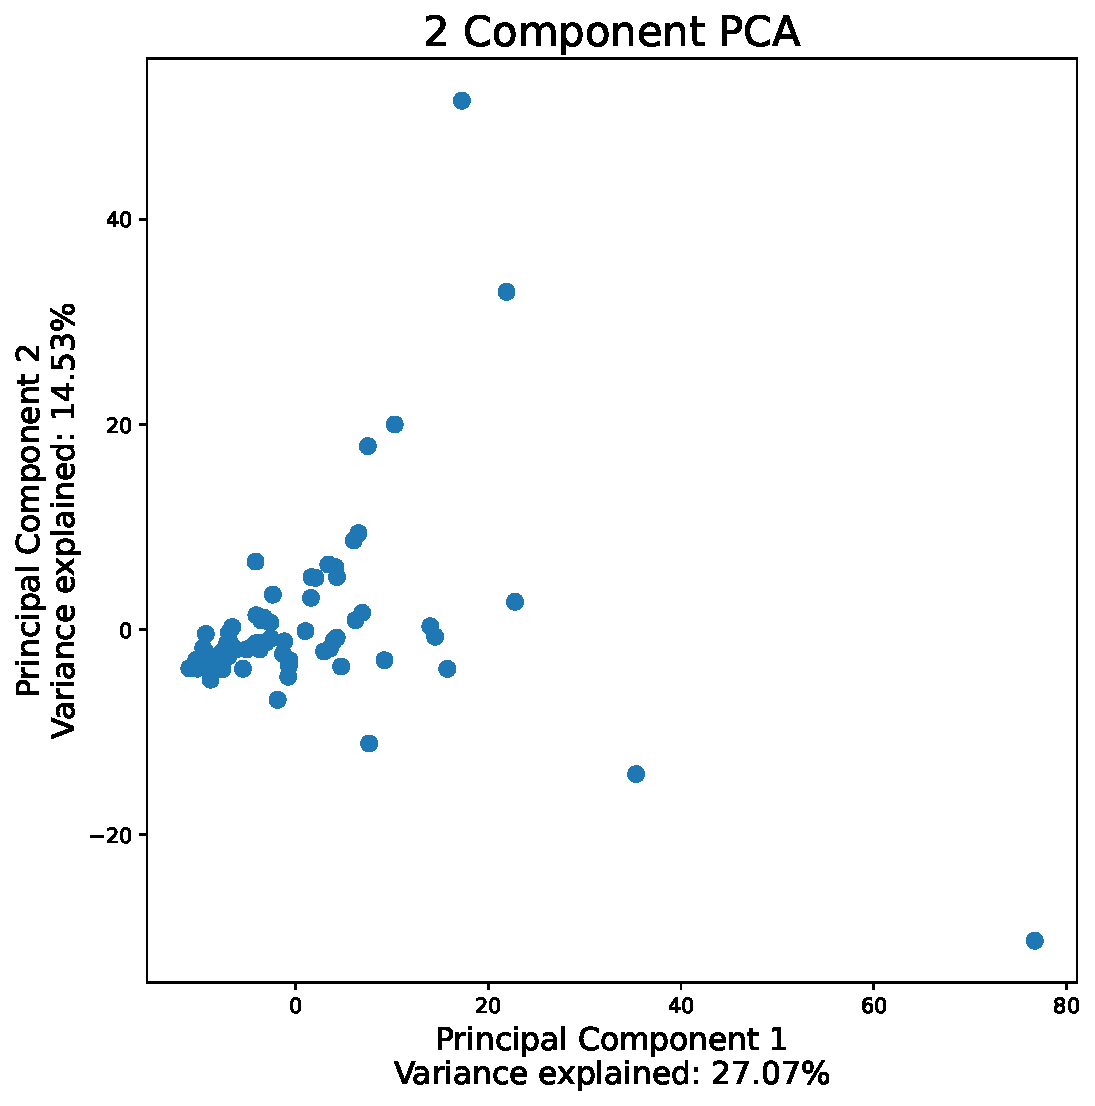
\includegraphics{tutorial_files/figure-pdf/perform_pca-output-1.pdf}

}

\end{figure}

\begin{itemize}
\tightlist
\item
  Interpretation of the PCA results:\\
  From the PCA results, we can see the first two PCs could explain about
  41\% of the variance in our data, which is not very high. We can also
  see that the samples are not well separated in the PCA plot, so we
  can't explain the group difference in dataset very well with the top 2
  features we have, which might be due to there is a non-linear
  relationship here in the features that couldn't be all explained by
  simply PCA analysis. Therefore, further non-linear analysis might be
  needed to better understand the relationship between the features and
  the samples. (I will add more functions to the package in the future
  to perform non-linear analysis, such as t-SNE, UMAP, etc.)\\
\end{itemize}

\begin{enumerate}
\def\labelenumi{\arabic{enumi}.}
\setcounter{enumi}{2}
\tightlist
\item
  (b)Next, we can do the same for the MA plot.\\
  The MA\_plot function will return a pandas dataframe containing the
  log2 fold change and the -log10 p-value\\
\end{enumerate}

\begin{Shaded}
\begin{Highlighting}[]
\NormalTok{MA\_plot}\OperatorTok{=}\NormalTok{sa.ma\_plot(normalized\_data)}
\end{Highlighting}
\end{Shaded}

\begin{figure}[H]

{\centering 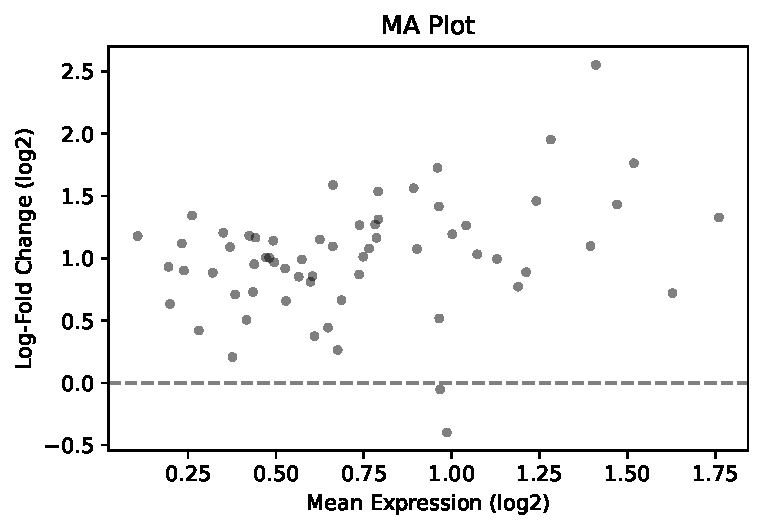
\includegraphics{tutorial_files/figure-pdf/perform_ma_plot-output-1.pdf}

}

\end{figure}

\begin{itemize}
\tightlist
\item
  Interpretation of the MA plot results:\\
  The MA plot shows that for most metabolites identified here, they were
  upregulated in the non-control group, which is an interesting
  observation here. It is about the idea that, for patients with
  disease, their metabolites profile might be different from the healthy
  people, and this difference might be due to they are unable to
  metabolize some metabolites (decreased liver function), or they are
  producing more metabolites than the healthy people. This is a very
  interesting observation, and we can further explore this in the
  future.\\
\end{itemize}

\begin{enumerate}
\def\labelenumi{\arabic{enumi}.}
\setcounter{enumi}{2}
\tightlist
\item
  (c)We can also do a volcano plot, which can show us the significantly
  differentially expressed metabolites in the data.\\
  The volcano\_plot function will return a pandas dataframe containing
  the log2 fold change and the -log10 p-value
  volcano\_plot=sa.volcano\_plot(normalized\_data)
\end{enumerate}

\begin{Shaded}
\begin{Highlighting}[]
\NormalTok{volcano\_plot}\OperatorTok{=}\NormalTok{sa.volcano\_plot(normalized\_data)}
\end{Highlighting}
\end{Shaded}

\begin{figure}[H]

{\centering 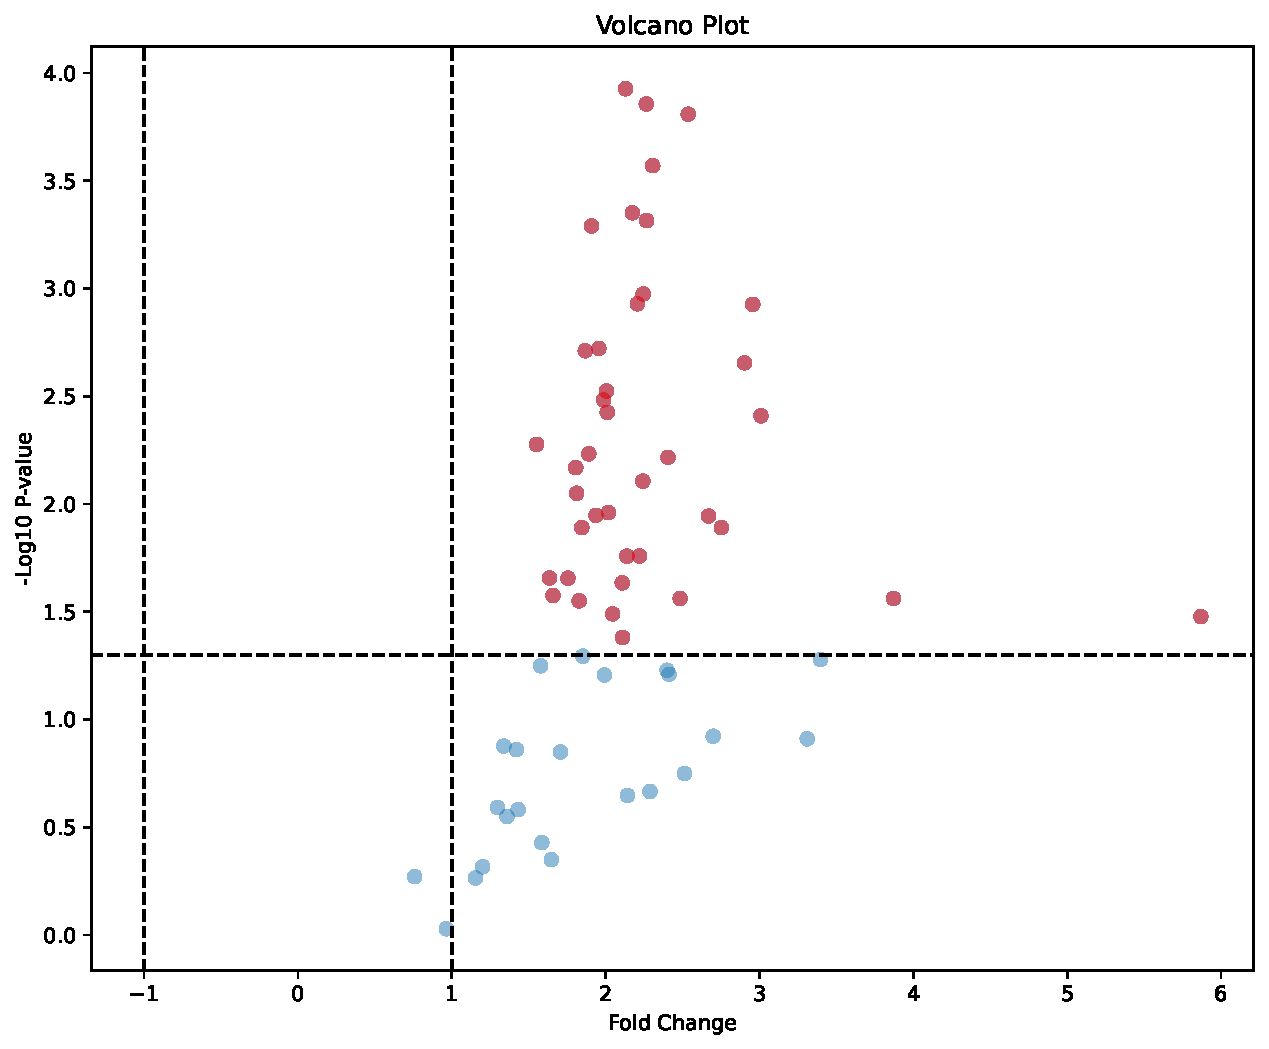
\includegraphics{tutorial_files/figure-pdf/perform_volcano_plot-output-1.pdf}

}

\end{figure}

\begin{itemize}
\tightlist
\item
  Interpretation of the volcano plot results:\\
  For the volcano plot here, every point represents a metabolite. The x
  axis represents the fold change of different metabolites, and y axis
  represents the adjusted p values using Benjamini-Hochberg method. The
  red points are the metabolites that are significantly different
  between the two groups, and the blue points are the metabolites that
  are not significantly different between the two groups. We can see
  that there are a lot of metabolites that are significantly different
  between the two groups, which is consistent with the MA plot results.
  We can also see that there are some metabolites that are not
  significantly different between the two groups, but they have a very
  high fold change, which is also interesting. We can further explore
  this in the future.\\
\end{itemize}

\textbf{Conclusion about applications of the tool}\\
- As we can see, using metabolomics analysis tools can help us process
the metabolites data and to better visually explore the metabolites as
features and metabolite expressions we have in different groups of
subjects, and help us to generate some interesting hypothesis that we
can further explore in the future.\\



\end{document}
